% Converted from reference/DRSFlare (MadCap Flare, Java target)

\chapter{db4o Replication System}
\label{drs:welcome}

The db4o Replication System provides functionality to periodically synchronize databases that work disconnected from each other. For example mobile devices synchronizing to a central server or desktop application.

The dRS can replicate between any number of db4o-databases. \hyperref[drs:db4o-replication-system-drs-db4o-databases-replication]{See "db4o to db4o Replication"} (p.~\pageref{drs:db4o-replication-system-drs-db4o-databases-replication})

Another feature is to replicate between VOD and db4o. \hyperref[drs:db4o-replication-system-drs-vod-replication]{See "Replication With VOD"} (p.~\pageref{drs:db4o-replication-system-drs-vod-replication})

Utilizing Hibernate dRS can also replicate between db4o and a RDBMS. \hyperref[drs:db4o-replication-system-drs-replication-with-rdbms]{See "Replication With Hibernate"} (p.~\pageref{drs:db4o-replication-system-drs-replication-with-rdbms})

\begin{center}
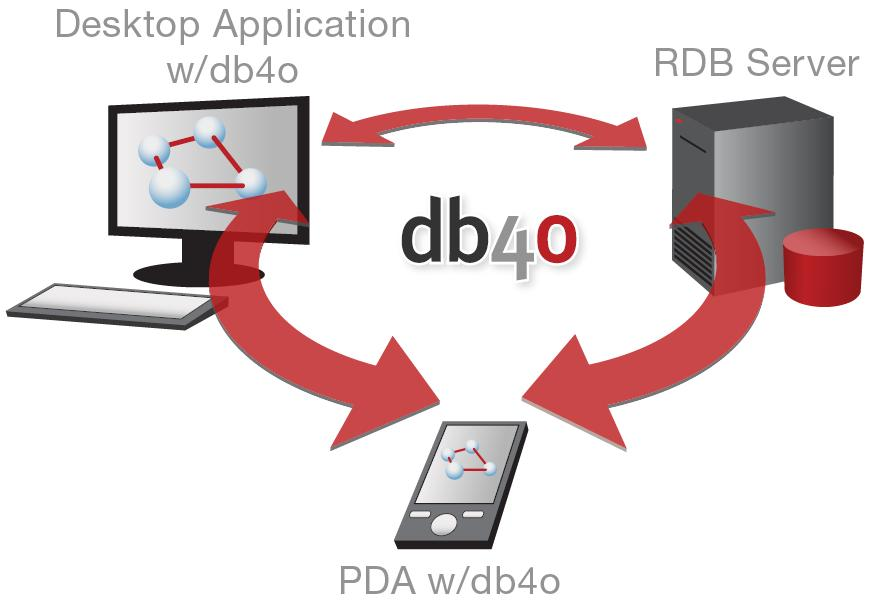
\includegraphics[width=\maxwidth]{images/drs-drsoverview.jpg}
\end{center}
The dRS source code is in the drs directory of the db4o repository at \href{https://github.com/blakemcbride/db4o}{\nolinkurl{github.com/blakemcbride/db4o}}.

